% Robotics Institute Technical Report
%
% Unofficial Template for RI Technical Reports
% Use with latex2e
%
% Modified by: David Fouhey, Oct 2014
% Created by: Daniel Morris, Dec 2000
%
% DM:
%   Since I was unable to find a template for Technical Reports, I made up my
%   own.  Use it at your own risk -- as I am not a latex guru.


\documentclass[twoside,10pt]{report}
\usepackage{marginnote}
\usepackage[left=1.5in,right=1.5in,top=1.5in,bottom=1.5in]{geometry}
\usepackage[usenames,dvipsnames]{xcolor}
\usepackage{graphicx,amsmath,amssymb,multirow,booktabs,color,verbatim,draftwatermark,cite,url,placeins}
\usepackage{algorithm, algpseudocode}
\usepackage[font=scriptsize]{subcaption}
\usepackage[font=scriptsize]{subfig}
\usepackage{layouts,array,wrapfig}
\usepackage[normalem]{ulem}
\usepackage{tgpagella}
\newcommand*{\QEDB}{\hfill\ensuremath{\square}}

%%%%%%%%%%%%%%%%%%%%%%%%%%%%%%%%%%%%
%DF: This needs to be removed to get 
%rid of all watermarks
\usepackage{draftwatermark}
\SetWatermarkText{DRAFT}
\SetWatermarkScale{0.5}
\SetWatermarkLightness{0.90}

%%%%%%%%%%%%%%%%%%%%%%%%%%%%%%%%%%%%
%DF: Nuke all the notes by using 
%the second note definition below
\newcommand{\note}[1]{\textcolor{red}{#1}}
%\newcommand{\note}[1]{}


%I usually like to put more figures on a page with text than latex's
%default
\renewcommand{\textfraction}{0.05}
\renewcommand{\topfraction}{0.9}
\renewcommand{\floatpagefraction}{0.8}
\DeclareMathOperator*{\argmin}{arg\,min}
\DeclareMathOperator*{\argmax}{arg\,max}


\newcommand{\clearemptydoublepage}{\newpage{\pagestyle{empty}\cleardoublepage}}

%Table of contents stuff
\setcounter{tocdepth}{1}

\begin{document}

% Adding notations
\newcommand{\fbold}{\mathbf{f}}
\newcommand{\supi}{^{(i)}}
\newcommand{\supj}{^{(j)}}
\newcommand{\zbold}{\mathbf{z}}
\newcommand{\subt}{_{1:t}}
\newcommand{\supR}{^{(R)}}
\newcommand{\Gbold}{\mathbf{G}}
\newcommand{\Obold}{\mathbf{O}}
\newcommand{\red}{\textcolor{red}}
\newcommand{\xbold}{\mathbf{x}}
\newcommand{\gbold}{\mathbf{g}}
\newcommand{\Xbold}{\mathbf{X}}
\newcommand{\xdbold}{\mathbf{x'}}
\newcommand{\ybold}{\mathbf{y}}
\newcommand{\xbvel}{\frac{\Delta \xbold}{\Delta t}}
\newcommand{\ybvel}{\frac{\Delta \ybold}{\Delta t}}
\newcommand{\xvel}{\frac{\Delta x}{\Delta t}}
\newcommand{\yvel}{\frac{\Delta y}{\Delta t}}
\newcommand{\subH}{_{t+1:t+H}}
\newcommand{\subti}{_{1:t-1}}
\newcommand{\xbvelinb}{\xbvel^{(i \in B_g)}}
\newcommand{\subtplus}{_{t+1}}
\newcommand{\supP}{^{(P)}}

%%% Local Variables:
%%% mode: latex
%%% TeX-master: "thesis"
%%% End:


\title{2 Legit 2 Quit}
\author{JJ Gibson}


%title page
\thispagestyle{empty}
%Put the date below the TR number
\date{}

\begin{center}

{\Huge \bf 2 Legit \\ 2 Quit} \\
\vspace{1cm}  
{\Large Anirudh Vemula} \\
\vspace{1cm} 

%%%%%%%%%%%%%%%%%%%%%%%%%%%%%%%%%
%Include in final thesis
%\vspace{-0.5cm}
%{\large CMU-RI-TR-00-00}
%\vspace{2cm}
%%%%%%%%%%%%%%%%%%%%%%%%%%%%%%%%%

{\Large July 2017} \\
\vspace{2cm}
{
\includegraphics[scale=0.3]{Figures/logo.eps}} \\
\vspace{1cm}
{\Large
  The Robotics Institute\\
  School of Computer Science \\
  Carnegie Mellon University\\
  Pittsburgh, Pennsylvania 15213\\
}
\vspace{1cm}
{\Large
{\bf Thesis Supervisors:}\\
Dr. Jean Oh\\
Dr. Katharina Muelling
}
\vspace{1cm}
\par ~ \\
{\large \it Submitted in partial fulfillment of the requirements \\for the degree of Master of Science in Robotics}
\vfill
{\large \copyright Anirudh Vemula, 2017}
\end{center}



%%% Local Variables:
%%% mode: latex
%%% TeX-master: "thesis"
%%% End:

\clearpage


%start the forematter 
\pagenumbering{Roman}
\clearemptydoublepage
\setcounter{page}{1}

\begin{centering} \section*{Abstract} \end{centering}
Group theory is pretty abstract, no?
\note{The last part of the thesis. Tie all the three papers into a single concise abstract.i}


\tableofcontents
\clearpage

%%%%%%%%%%%%%%%%%%%%%%%%%%%%%%%%%
%Include in final thesis
%\clearpage \listoffigures
%\clearpage \listoftables
%\clearpage
%%%%%%%%%%%%%%%%%%%%%%%%%%%%%%%%%

%start the actual document
\pagenumbering{arabic}
\setcounter{page}{1}


\chapter{Introduction}
\label{chap:introduction}
In this chapter, we will motivate the problem tackled by this thesis and highlight the challenges involved. We will then present necessary background to understand the rest of the thesis by formally laying out the problems of path planning and trajectory prediction. We finish the chapter by describing the organization of the thesis. 

\section{Planning and Dynamics}
\label{sec:intro-motivation}

Navigation is an essential task for the autonomous mobile robot. The task not only involves how the robot can move on its own, but also how to achieve various goals and objectives. Specifically, the robot has to achieve its goals in the presence of hard constraints such as dynamic feasibility, collision avoidance, and soft constraints such as social compliance. These problems involve finding trajectories in the workspace from a start configuration to a goal configuration that satisfy the aforementioned constraints. \textit{Path Planning} is the problem of finding such a trajectory. The path planning approach depends on two important properties of the planner: The agent needs to have an accurate model of the dynamics of the environment or state of the world around it, and it needs to have a model of how its actions affect the world state. For mobile robots, this is significantly challenging as they have to rely on perception to create a model of the world state. In the absence of an accurate long-horizon models and limited perception, mobile robots were traditionally relegated to use reactive methods or one-step planning algorithms, \cite{fox1997dynamic,brock1999high}. These reactive methods map the observed state of the world at the current time-step to an action for the robot to execute. Employing an accurate model of the environment, the mobile robot can instead plan its actions ahead, to achieve more efficient (in some cases, more social) behavior. However, the major challenge in achieving this objective is modeling the state of the environment, which can be dynamic.

Dynamics is an important aspect of mobile robot navigation in partially known or completely unknown environments. Robot dynamics are the kinematic and dynamic constraints that need to be considered while planning the path of the robot. Most modern planning algorithms consider these kinodynamic constraints to come up with feasible trajectories for the robot to execute. The other kind of dynamics in navigation is, dynamics of the world or environment. An environment where other agents or obstacles move is said to be dynamic. A major challenge in navigation is to come up with an accurate model for their motion, so that it can be accounted while planning the path of the robot. Such a model needs to result in accurate long-term predictions of the trajectories of other agents in the environment. More often than not, dynamics of the environment are not readily predictable and need to be supplemented by sensory information. Given sensory information regarding the past behavior of the agents, the model needs to predict their future behavior.

In this thesis, we focus on the problems of planning and modeling dynamics. More specifically, the first part of the thesis deals with  path planning in dynamic environments and the latter half deals with human trajectory prediction in dense crowds. We present novel solutions and take a small step towards making the goal of autonomous mobile robot navigation more realizable.

\section{Motivation}
\label{sec:intro-motiv-chall}

We envision mobile robots to coexist with humans in unscripted environments and accomplish various kinds of tasks. Existing works towards this goal started out in the 1990s with RHINO, \cite{thrun99}, and MINERVA, \cite{Thrun2000ProbabilisticAA}, both designed as interactive museum tour guide robots that will move among humans in museums. These works made extensive use of path planning, localization and mapping methods that were developed around the same time. These works pioneered the field of service robots inciting a period of exciting research in the area of robot navigation in human crowds. Chapter \ref{chap:survey} discusses several of the subsequent works.

Despite the decades of research towards this goal, there are several fundamental problems that remain unsolved. Traditional algorithms for navigation in dynamic environments tend to make strong assumptions about the environment and its own motion model, in order to efficiently plan paths quickly \cite{lavalle2006planning, latombe2012robot}. These planning algorithms don't extend readily to unscripted environments where the agent is highly uncertain about the dynamics of the environment. Most of the works towards modeling dynamics of an unknown environment make simplifying reductions such as independence of motion and the number of surrounding agents \cite{choset2005principles}. Situations where the actions of each agent affect that of the other (especially, in the case of human-robot interaction) are not modeled. To make the vision of coexisting robots and humans a reality, there is a great need for efficient planning algorithms in dynamic environments and accurate models for environment dynamics.

\section{Problem Definition}
\label{sec:intro-background}

In this section, we describe the formal problem definitions for the path planning and trajectory prediction problems. Subsequently, we describe how planning can be reduced to inference in a joint prediction model and briefly present the \textit{freezing robot problem}, which was first introduced in \cite{trautman10}.

%\subsection{Notation}
%\label{sec:intro-notation}

%For the rest of this thesis, we will adhere to the following notation:
%\begin{itemize}
%\item $G$ : Graph representing a discretized state-space that is searched
%\item $S$ : Set of discretized states in the search space
%\item $T$ : Set of feasible transitions between any two states in $S$
%\item $c$ : Cost function encoding the cost of each transition in $T$
%\item $X_s$ : Start state (an element of $S$)
%\item $X_g$ : Goal state (an element of $S$)
%\item $\pi(X_i, X_j)$ : A path in $G$ between two states $X_i$ and $X_j$ in $S$ using $T$
%\item $\pi^*(X_i, X_j)$ : Minimum cost path in $G$ between states $X_i$ and $X_j$
%\item $\epsilon$ : Heuristic inflation factor
%\item $\fbold$ : Trajectory as a mapping from discrete time-step $t$ to $(x,y) \in \mathbb{R}^2$ in continuous space
%\item $\zbold$ : Observed locations in $\mathbb{R}^2$ at discrete time-steps
%\item $g$ : Goal location in continuous $\mathbb{R}^2$ space
%\end{itemize}

\subsection{Path Planning Problem}
\label{sec:intro-path-plann-probl}
The general path planning problem for an explicit goal configuration is, given the robot dynamics, its start configuration and the configuration space, to find a path that is collision-free, dynamically feasible to execute and is a solution.


Let $X \subset \mathbb{R}^n$ be the configuration space of the system. Let $X_{obs} \subset X$ be invalid configurations that result in collision with obstacle. The dynamics of the system is specified as a dynamics constraint $g(x, \frac{dx}{dt}, \dots, \frac{d^rx}{dt^r}) \leq 0, x \in X$, where $r$ is the relative degree. Let the trajectory $\xi: [0, 1] \rightarrow X$ be a continuous mapping from time to configuration. The planning problem is to find the shortest dynamically feasible trajectory from start $x_0$ to the goal $x_f$ that is collision free. This is expressed as follows:

\begin{equation}
\begin{aligned}
\label{eq:planning-problem}
& \underset{x(t)}{\text{minimize}} & & \int\limits_0^1 \| \dot{x}(t) \| \mathrm{dt} \\
& \text{subject to} & & x(0) = x_0 \\
&                   & & x(1) = x_f \\
&                   & & g(x, \frac{dx}{dt}, \dots, \frac{d^rx}{dt^r}) \leq 0 \\
&				    & & x(t) \in X \setminus X_{obs}, t \in [0,1] \\
\end{aligned}
\end{equation}

The above optimization problem seeks to find the shortest trajectory between the start and goal configuration. In the presence of a cost function $c(x_i, x_j)$ that encodes the cost of transition from $x_i$ to $x_j$, the objective of the optimization can be changed appropriately.

\subsection{Trajectory Prediction Problem}
\label{sec:intro-traj-pred-probl}

Trajectory prediction in a dynamic environment entails predicting the future trajectories of all dynamic agents in the environment until a fixed horizon. As argued before, this problem is challenging as we need to model the world dynamics to obtain accurate predictions.

Given a dynamic environment with agents indexed by the set $\{1, 2, \cdots, N\}$, where $N$ is the number of agents in the environment. The trajectory of agent $i$ is given by $\fbold^{(i)} = (f_1^{(i)}, f_2^{(i)}, \cdots, f_T^{(i)})$ where $T$ is the length of trajectory, and $f_t^{(i)}$ represents the location of agent $i$ at time $t$. We also assume that we have access to their past observed locations given by $\zbold$, where $\zbold^{(i)} = (z_1^{(i)}, z_2^{(i)}, \cdots, z_t^{(i)})$ are the observed locations of agent $i$ until time $t$. \\



The trajectory prediction problem is to model the following joint distribution
\begin{equation}
  \label{eq:traj-prediction-problem}
  P(\fbold^{(1)}, \fbold^{(2)}, \cdots, \fbold^{(N)} | \zbold^{(1)}, \zbold^{(2)}, \cdots, \zbold^{(N)})
\end{equation}
i.e., given their observed locations $\zbold^{(1)}, \zbold^{(2)}, \cdots, \zbold^{(N)}$, we want to estimate the distribution over their trajectories until some future time $T$. Note that such joint modeling accounts for dependencies between trajectories of different agents which, as we show later, is paramount for accurate predictions.

\subsection{The Freezing Robot Problem}
\label{sec:intro-plann-as-infer}
%\label{sec:intro-freez-robot-probl}

The freezing robot problem, first introduced in \cite{trautman10}, highlights the deficiencies of existing predictive models that force the robot to come to a complete stop (or freeze). \cite{trautman10} shows that even under \textit{perfect individual prediction} for all agents in the environment, the freezing robot problem can occur for certain configurations. Figure \ref{fig:intro-freeze} shows a common scenario in human crowds, where people walking shoulder-to-shoulder towards the robot, forces it to go around the crowd or in the worst case, stop completely.
% As in \cite{trautman10}, this happens as most navigation approaches ignore mathematical models of cooperation between humans and the robot.
As shown in \cite{trautman10}, this happens as most existing navigation approaches ignore implicit cooperation between humans and the robot. 

\begin{figure}
  \centering
  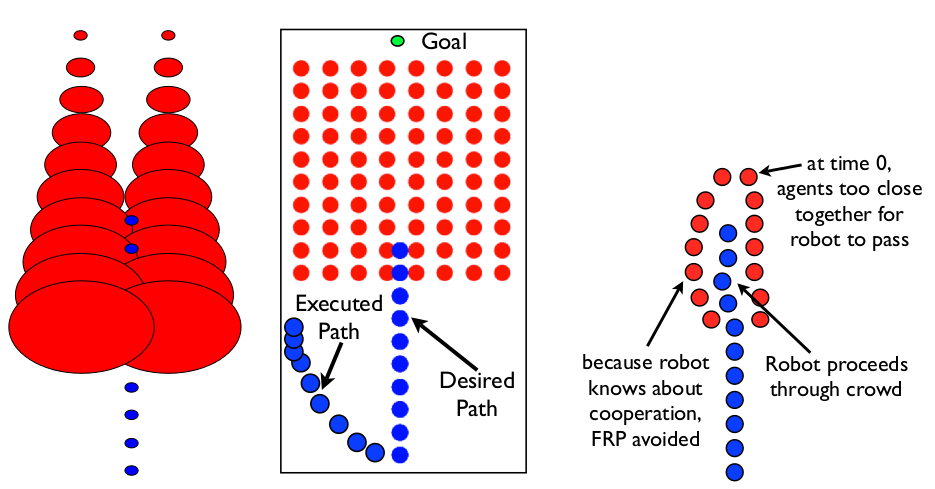
\includegraphics[width=\linewidth]{Figures/frp.png}
  \caption{Example of Freezing Robot Problem, \cite{trautman10}}
  \label{fig:intro-freeze}
\end{figure}

The key insight, which we will follow in this thesis, is that agents engage in \textit{joint collision avoidance}, i.e. they adapt their trajectories to make room for other agents to navigate. The joint collision avoidance criteria has been shown to improve tracking of humans in dense crowds, \cite{pellegrini09, trautman10, trautman13, trautman15}.

The approach, suggested in \cite{trautman10}, to solve the freezing robot problem is to move away from individual agent prediction and model the joint distribution of trajectories, as shown in equation \ref{eq:traj-prediction-problem}. In addition to joint modeling, we need to model the robot as one of the agent so that we also include interactions between the robot and other agents. In other words, the prediction algorithm should model
\begin{equation}
  \label{eq:freeze}
  P(\fbold^{(R)}, \fbold^{(1)}, \fbold^{(2)}, \cdots, \fbold^{(N)} | \zbold^{(1)}, \zbold^{(2)}, \cdots, \zbold^{(N)})
\end{equation}
where $\fbold^{(R)}$ is the robot's trajectory. Note that this distribution encodes the idea of \textit{cooperative planning} as it captures interactions among agents and the robot.

An interesting outcome from this modeling is that planning the robot's trajectory reduces to inference in this joint model, i.e. inferring what the robot should do given the actions of other agents.
\begin{equation}
  \label{eq:planning-reduced-to-inference}
  (\fbold^{(R)}, \fbold^{(1)}, \cdots, \fbold^{(N)})^* = \argmax_{(\fbold^{(R)}, \fbold^{(1)}, \cdots, \fbold^{(N)})} P(\fbold^{(R)}, \fbold^{(1)}, \cdots, \fbold^{(N)} | \zbold^{(1)}, \cdots, \zbold^{(N)})
\end{equation}

As we will see in Chapter \ref{chap:oigp}, this results in ``human-like'' behavior for the robot when modeling crowds, as we model the robot as one of the humans. 


\section{Thesis Organization}
\label{sec:intro-thesis-organization}

The remainder of this thesis is organized as follows: Chapter \ref{chap:survey} presents a brief survey of past works in the domain of robot navigation in human crowds. We also list out several works in the domain of human tracking in crowds and video surveillance. Chapter \ref{chap:ppad} presents our novel approach to solving the problem of efficient path planning in dynamic environments when an accurate model of the world dynamics is known. We propose a heuristic-based graph search algorithm that results in safe and feasible paths for the robot in short planning times. Additionally, we present theoretical guarantees on the optimality of the resulting path and completeness of the planning algorithm. The task of obtaining an accurate model of the world dynamics (specifically, crowd dynamics) is tackled in Chapter \ref{chap:oigp} where we propose a novel statistical modeling approach that couples predictions for multiple agents through occupancy grids. The proposed model is learned from real world trajectory and can be used to predict future trajectories of dynamic agents in an environment. Finally, Chapter \ref{chap:conclusion} summarizes the contributions of this thesis and provides directions for future research in this area.

%%% Local Variables:
%%% mode: latex
%%% TeX-master: "thesis"
%%% End:


\clearpage

\chapter{A Survey of Navigation in Human Crowds}
\label{chap:survey}
In this chapter, we present a brief survey of past literature in the domain of robot navigation in human crowds. To address this problem, these works either assume or construct a model of human motion which is used to predict future trajectories. Given these predictions, they then proceed to plan the path for the robot to navigate through the crowd to its destination. Thus, the efficacy of these approaches depend on the accuracy of their human future trajectory predictions and robot path planning algorithms. As a part of this survey, we will present these aspects of the approaches in the context of our problem.

There has been a diverse set of works over the past two decades that have tackled the problem of robot navigation in human crowds. These approaches make varied assumptions, have different objectives and exhibit a wide range of results. We try to broadly classify these approaches according to their methodology, and highlight the benefits and drawbacks. More specifically, we will categorize the approaches based on their modeling assumptions and their planning objective. For each category, a brief description of the employed methodology is discussed in addition to its advantages and disadvantages. The intent of this chapter is to present the landscape of past research in this field to give some perspective and context to our proposed work presented in the coming chapters.

\section{Taxonomy of Approaches}
\label{sec:survey-taxonomy-approaches}

We broadly classify past works on the basis of their (1) objective of the planning algorithm, and (2) human motion model to predict future trajectories. The resulting classes are described in the following subsections.

\subsection{Planning Objective}
\label{sec:survey-planning-objective}
Planning the robot's path through the crowd involves several constraints that need to be satisfied. Collision-avoidance, dynamic feasibility and social compliance are some such constraints that typical path planning algorithms consider. Collision-avoidance is self-explanatory in that it requires the robot to move such that it avoids collision with any obstacles including other agents in the crowd. Dynamic feasibility implies that the path planned needs to be feasible for the robot to execute with its dynamics and motion model. In contrast, social compliance is a complex constraint that is hard to rigidly define. In broad terms, it implies that the resulting path for the robot needs to adhere to social norms followed by humans, thus making the path interpretable and predictable for humans in the crowd. Given these constraints, we can broadly classify past works as follows:

\subsubsection{Safe Robot Navigation}
\label{sec:survey-safe-robot-navig}

The objective of these set of works involve the task of navigating a robot safely through a human crowds avoiding collisions and planning a dynamically-feasible path. As a result, these works do not consider the social aspects of navigation and hence, the resulting path of the robot is safe but may not be ``human-like''.

\subsubsection{Social Robot Navigation}
\label{sec:survey-soci-robot-navig}

These works tackle the more difficult objective of not only safe robot navigation (as above), but also to move in a socially compliant way. Thus, the resulting robot paths are more predictable for the surrounding humans in the crowd.

\subsubsection{Trajectory prediction}
\label{sec:survey-traj-pred}

The set of works in this class do not necessarily involve robot navigation, but rather tackle the problem of accurately modeling human trajectories in crowds. As shown in Section \ref{sec:intro-plann-as-infer}, planning the path for the robot reduces to inference in this model, thereby obtaining a path for the robot that is ``human-like'' or socially-compliant. Most of the works in this category are from the domain of video surveillance tracking and computer vision.



\subsection{Human Motion Model}
\label{sec:survey-human-motion-model}

For robots to navigate in human crowds, they need to employ a model of human motion in crowds so that accurate predictions of their future trajectories can be made. These predictions are then fed into a planning algorithm to plan the final trajectory for the robot to follow to navigate through the crowd. We can broadly classify past works based on the human motion model employed as,

\subsubsection{Independent Handcrafted Model (IH)}
\label{sec:survey-indep-handcr-model}

These approaches model each agent (or human) in the crowd independently of each other, i.e. they assume that the predictions for human trajectories are mutually independent. In addition to this assumption, the motion model is handcrafted (like a rule-based model) to match social behavior usually observed in crowds.

\subsubsection{Independent Trained Model (IT)}
\label{sec:survey-indep-train-model}

Similar to the IH category, works in this class make the independence assumption but the model, instead of being handcrafted, is learned by training it on real-world human trajectory data.

\subsubsection{Joint Handcrafted Model (JH)}
\label{sec:survey-joint-handcr-model}

Unlike the independent models, these works assume that the predictions are dependent on each other and jointly predict the trajectories of all interacting humans in the crowd. Most of these approaches don't model the joint distribution of trajectories explicitly, instead use some approximate handcrafted potential terms to capture the interactions.

\subsubsection{Joint Trained Model (JT)}
\label{sec:survey-joint-trained-model}

Similar to the JH class of works, these approaches jointly predict the trajectories of all humans in the crowd but the joint distribution is learned from real-world human trajectory data, and the learned model is used at inference time to make predictions. \\




In each of the categories in the above taxonomy, there are several related works. For conciseness purposes, we describe only the latest works that have been shown to perform better than others in their respective category. We would like to point out that our list of works is not exhaustive and doesn't list all the related past approaches. The taxonomy and the related works have been summarized in table \ref{tab:taxonomy}.

\begin{table}[H]
  \centering
  \begin{tabular}{|p{5cm}|p{1.5cm}|p{1.5cm}|p{1.5cm}|p{1.5cm}|}
    \hline
     & \textbf{IH} & \textbf{IT} & \textbf{JH} & \textbf{JT}\\
    \hline
    \textbf{Safe robot navigation} & \cite{hoeller2007accompanying} & \cite{aoude2013probabilistically}& \cite{trautman15} & \cite{kim2014brvo} \\
    \hline
    \textbf{Social robot navigation} & \cite{kirby2009companion} & \cite{kim2016socially} & \cite{shiomi2014towards} & \cite{Kretzschmar16} \\
    \hline
    \textbf{Trajectory prediction} & \begin{center}{\textbf{-}}\end{center} & \cite{joseph2011bayesian, kitani2012activity} & \cite{luber2010people} & \cite{pellegrini2010improving, alahi16} \\
    \hline
  \end{tabular}
  \caption{Taxonomy of related works}
  \label{tab:taxonomy}
\end{table}

\section{Safe Robot Navigation}
\label{sec:survey-safe-robot-navig-1}

As described in the above section, the objective of these works is to navigate a robot through human crowds avoiding collisions and satisfying dynamic feasibility. Early works have dealt with this problem by using traditional handcrafted human motion models to obtain predictions for future trajectories. Most of these models make the simplistic assumption that motion of agents are independent of each other, except in close quarters where handcrafted potential terms predict collision-avoidance.

\cite{hoeller2007accompanying} employs a laser-based tracker to track humans in the crowd and combines the estimates with a potential field-based model to predict their future motion. These models have handcrafted quadratic repulsive potential terms that result in predictions that avoid obstacles and linear attractive potential terms that steer the predictions towards destination. These potentials are a function of the distances to other humans, obstacles and destination. Given these predictions of future trajectories, the path of the robot is planned using a variant of Expansive space trees (EST), \cite{hsu02}.

The potential field-based model captures simplistic human-space interactions such as obstacle avoidance, and works well in wide open spaces. The linear attractive potential terms capture the intent of the human to go towards the destination, but require the knowledge of the true destination of every human in the crowd. Although they are capable of modeling obstacle avoidance, they fail at accurately capturing complex human-human interactions like cooperation. Another major drawback of such approaches is due to the independence assumption that doesn't account for the effect of robot's actions on the human trajectories.

On the other hand, \cite{aoude2013probabilistically} uses similar independent human motion models but learned from real pedestrian data, rather than using handcrafted potential terms. The learned models are used to forecast future trajectories for humans in the crowd. More specifically, \cite{aoude2013probabilistically} use Gaussian Processes (GP) to learn independent models of motion patterns of humans in real crowds. The future trajectories are grown using a variant of RRT to follow the motion pattern. Chance-constrained RRT, \cite{luders10}, is used to plan the robot's path guaranteeing probabilistic robustness to predicted human paths. The GP model is trained on human trajectories from real annotated crowd data.

Learning motion patterns from data enables \cite{aoude2013probabilistically} to result in predictions that capture several navigation behaviors. By combining GPs and RRTs, it has a run-time that is suitable for real-time operation. Chance-constrained RRT, used in planning the path of the robot, guarantees probabilistically safe trajectories for the robot in the presence of humans. But the motion patterns modeled account for each individual human individually and do not capture human-human interactions. In dense crowds, where such interactions play a major role such a model would result in inaccurate predictions.

More recently, there have been several works which move away from the independence assumption and model the future trajectories of all interacting agents as a joint distribution. As a result, these works can capture human-human interactions within the crowd. \cite{trautman15} introduced \textit{Interacting Gaussian Processes} (IGP), which uses GPs to model individual trajectories of the pedestrians (and the robot) and couples their predictions using a handcrafted interaction potential term that aims to capture joint behaviors, such as cooperative collision avoidance. The robot's path is chosen as the MAP assignment to the modeled joint distribution (similar to Section \ref{sec:intro-plann-as-infer}).

The handcrafted interaction potential term explicitly assigns low probability mass to predictions that result in human-human and human-robot collisions, thus capturing joint collision avoidance. One important contribution of this work is that since the robot is part of the joint model, it also accounts for human-robot cooperation which was lacking in previous works. A major drawback of such an approach is the hand-tuned potential term that doesn't generalize across different environments and crowd settings.

To account for this drawback, one needs to learn the joint distribution from real-world crowd data without using hand-tuned potential terms. \cite{kim2014brvo} introduced an online motion prediction method that learns per-agent motion models as the robot moves, with no prior knowledge of the environment. The prediction algorithm extends the reciprocal velocity obstacles approach, \cite{van2008reciprocal}, which captures joint collision avoidance among pedestrians. Given the predictions, the robot plans its own path using generalized velocity obstacles method, \cite{wilkie2009generalized}.

By learning individual motion model for each observed pedestrian, the online motion-prediction model can perform better than less responsive offline motion models. But the reciprocal velocity obstacles approach can only capture collision avoidance behavior and not cooperative behavior that is commonly observed in crowds. Also, the predictions are accurate only for short-term horizons and worsen over longer horizons.


\section{Social Robot Navigation}
\label{sec:survey-soci-robot-navig-1}

Works in this category tackle the problem of coming up with socially-compliant paths in addition to safe and dynamic-feasibility. Social compliance implies that the resulting paths are predictable for surrounding humans in the crowd, which can be a difficult to define as an objective. Early works in this domain use rule-based systems which try to capture social norms that are typically observed in crowds.

\cite{kirby2009companion} presents an approach that tracks surrounding humans and uses the estimate of their current velocity to predict future locations. Pre-defined social conventions such as person avoidance, personal space, pass on the right, keeping a constant velocity etc. are encoded as social constraints on the robot's path. Given these constraints, A* is used to plan the robot's path. Since social norms such as passing on right and respecting personal space are explicitly encoded into the planning, the resulting path has social compliance respecting such behaviors. On the other hand, the constant velocity assumption used in human motion prediction doesn't hold true in real crowds and the pre-defined social conventions are specific to office hallways, not for general settings.

Rather than using these handcrafted rules to define social conventions, \cite{kim2016socially} learns social behaviors from human demonstrated crowd navigation behavior. They employ Bayesian inverse reinforcement learning (IRL), \cite{Ramachandran2007BayesianIR}, to learn a cost function from human demonstrations obtained by tele-operating the robot in a real crowd. The features used to characterize this cost function are pedestrian speed, direction of his motion, local crowd density and distance to goal, and these are extracted from raw RGB-D sensor data. A low-level local path planner is used to optimize the cost function and plan an optimal path for the robot.

As the cost function is learned from human demonstrations, the robot learns to navigate in a socially compliant way and is generalizable to new environments. A reactive planner is used to account for any uncertainty regarding the pedestrian motion, which replans every time new sensor data is obtained. The major drawback of this approach is that future motions of the humans are independent of each other and hence, cannot capture human-human and human-robot interactions.

As argued before, to capture these interactions we need to model the joint distribution of the trajectories. \cite{shiomi2014towards} approximates this distribution by using a variant of the social forces model, \cite{helbing95}, which describes the interactions in terms of forces that correspond to objectives. Attractive forces guide the pedestrians towards their goal whereas repulsive forces ensure that collisions are avoided. These forces are a function of positions and speeds of the pedestrians. Given the predictions, the robot's path is planned using a local reactive planner.

In sparse crowds, approaches such as \cite{shiomi2014towards} that employ the social forces model have been shown to result in socially compliant paths. But in dense crowds, social force models fail as they cannot capture complex crowd behavior such as cooperation. This restricts the applicability of such approaches in dense crowds.

\cite{Kretzschmar16} learns parameters of a joint distribution model over all interacting agents using Maximum Entropy IRL, \cite{Ziebart2008MaximumEI}, from human demonstrations. The features used include acceleration, velocity, clearance, collision-avoidance, passing left vs right, group behavior etc. During prediction, they explicitly account for interactions between humans, and predict the future paths of both the humans and the robot jointly. Since the cost function is learned from real crowd data and the future paths are jointly predicted, this approach can capture interactions that are commonly seen in dense crowds resulting in socially compliant path for the robot. Interestingly, the model also learns cooperative behavior between the humans and the robot. The major drawback is that the dimensionality of the feature vector scales with the number of agents in the crowd, making the approach scale poorly with the size of the crowd.

\section{Trajectory Prediction}
\label{sec:survey-traj-pred-2}

In this section, we will discuss works in the domain of video surveillance tracking and human trajectory prediction in crowds. These works are relevant as predicting trajectories of surrounding humans accurately is highly important to the task of navigation through crowds. Given such an accurate prediction model, we can plan the path of the robot using the same model to obtain socially-compliant paths that are ``human-like''. 

Some of the works such as \cite{joseph2011bayesian} learn independent human motion prediction models by modeling motion patterns of pedestrians in real crowds. These motion patterns are modeled using GPs to regress over their $(x,y)$ positions and a Dirichlet process (DP) to account for the unknown number of motion patterns. Activity forecasting introduced in \cite{kitani2012activity}, on the other hand, infers traversable regions in a scene by modeling human-space interactions using semantic scene information. The traversability is defined through a cost function that is learned using Maximum Entropy IRL, \cite{Ziebart2008MaximumEI}, over the static semantic environment map from human trajectories.

Approaches that model motion patterns of pedestrians in environments capture human navigation behaviors and implicitly model environmental constraints on human motion (such as a static obstacle in the environment, that pedestrians avoid). Similarly, approaches like \cite{kitani2012activity} that explicitly model human-space interactions can learn more refined constraints on the motion according to the semantic objects in the environment. Unfortunately, both these sets of approaches don't account for human-human interactions i.e. they model each human independently of each other. Hence, they cannot capture cooperation or high-level social behavior among humans in the crowd.

As we already know, to account for human-human interactions we need to jointly predict the trajectories of all interacting agents in the crowd. \cite{luber2010people} presented a pedestrian dynamics model based on Social Forces, \cite{helbing95}, that integrates the social forces model with a Kalman filter based multi-hypothesis tracker. The resulting model accounts for both inter-person influences and influences from static obstacles (using an occupancy map) in the environment. Thus, the trajectory predictions are accurate for humans in real crowds. One of the several drawbacks of such an approach, as discussed in the previous section, is that the use of social forces model has been shown to be effective only in sparse crowds and not in dense crowds. This makes it not readily applicable for any crowd scenario. Another important drawback of the model is that, as it doesn't infer the destination of the pedestrian, its long term prediction accuracy is low (Note that attractive forces that guide the pedestrian to the destination, which are a part of social forces, aren't used in this approach).

More recently, there have been approaches that learn a joint distribution over future trajectories of all interacting agents from real crowd data, rather than using handcrafted potential terms or forces. \cite{pellegrini2010improving} introduces a third order conditional random field (CRF) based approach to model the joint distribution of trajectories. The CRF-based approach is also able to identify groups within crowds on the basis of past trajectories. The parameters of the CRF are learned by training the model on annotated crowd datasets with very dense crowds. Taking a similar approach, \cite{alahi16} presents an LSTM-based approach that learns a deep recurrent generative model of the joint distribution accounting for interactions and short-term intentions. Given the past trajectories of all agents, this model couples their predictions through a \textit{social pooling} layer that combines the hidden states of neighboring pedestrians.

These joint data-driven approaches perform well in real world dense crowd trajectory prediction tasks and capture important social aspects such as cooperation, joint collision avoidance and group memberships. Two important drawbacks of this approach are, (1) the human-space interactions, such as static obstacle avoidance, are not included in the model, and (2) they work only for short horizons as they are aimed to model interactions rather than achieve accurate long term predictions.

\section{Summary}
\label{sec:survey-summary}

In this chapter, a brief survey of past literature in the domain of navigation and trajectory prediction in human crowds is presented. Approaches ranging from independent modeling with rule-based models to joint modeling using deep recurrent networks have been discussed along with their applicability and shortcomings. The intent of this chapter is to get a better understanding of the work that has been done and how that leads up to the work presented as a part of this thesis.

In the next chapter, Chapter \ref{chap:ppad}, we present a novel planning algorithm that enables robots to navigate crowded dynamic environments where the path of the dynamic obstacle is known. Such an algorithm can be used on a robot to re-plan its path upon receiving new sensory information and subsequent dynamic obstacle trajectory predictions. The problem of predicting the trajectory (especially, that of humans in crowds) is tackled in Chapter \ref{chap:oigp}, where we present a statistical model that, given the past trajectories, predicts future trajectories accurately for long horizons.

%%% Local Variables:
%%% mode: latex
%%% TeX-master: "thesis"
%%% End:


\clearpage

\chapter{Path Planning in Dynamic Environments}
\label{chap:ppad}
\note{This chapter should be adapted from SoCS 2016 paper.}
%%% Local Variables:
%%% mode: latex
%%% TeX-master: "thesis"
%%% End:


\clearpage

\chapter{Human Trajectory Prediction in Dense Crowds}
\label{chap:oigp}
In this chapter, we will present a novel trajectory prediction algorithm for humans in dense crowds assuming we have access to their past trajectories. The presented algorithm tries to capture human-human interactions such as joint collision avoidance and cooperation. More specifically, we develop an approach that models the joint distribution over future trajectories of all interacting agents in the crowd, through a local interaction model that we train using real human trajectory data. The interaction model infers the velocity of each agent based on the spatial orientation of other agents in his vicinity. During prediction, our approach infers the goal of the agent from its past trajectory and uses the learned model to predict its future trajectory. We demonstrate the performance of our method against a state-of-the-art approach on a public dataset. Results show that our model outperforms when predicting future trajectories for longer horizons. This chapter is adapted from our paper \cite{VemulaMO17} presented at ICRA 2017.

\section{Introduction}
\label{sec:oigp-introduction}

There is an increasing need for robots to operate in the midst of
human crowds. This requires the robot to be able to navigate through a
crowd in a socially compliant way, i.e., the robot needs to
collaboratively avoid collisions with humans and adapt its
trajectories in a human predictable manner.

To date, the majority of existing works in the area of social
navigation has focused on the prediction of individual motion patterns
in the crowd to improve the navigation performance~\cite{thompson09,
  bennewitz05, large04}. However, even in the case of perfect
prediction, these approaches can lead to
severely suboptimal paths \cite{trautman10}.
The primary reason for such underperformance is that these approaches
do not capture the complex and often subtle interactions that take
place among humans in a crowd; that is, these approaches model each
agent independently of the others. This observation leads to the
insight that agents in crowds engage in joint collision avoidance.

Humans navigate through dense crowds by adapting their trajectories
to those of other people in the vicinity.
Figure~\ref{fig:oigp-intro} shows three examples of such behavior where
people pass through, slow down, or go around when they are near
other pedestrians.
In order to learn to navigate in a socially compliant way, it is key
to capture such human-human interactions observed in a crowd.

Pioneering works by~\cite{helbing95,hall63} propose hand-crafted
functions to model such interactions based on proximity. Such
functions are, however, limited in the complexity of interactions that
they can model and fail to generalize for crowded settings. Trautman
et. al. \cite{trautman10} proposed an approach that explicitly models
human-human and human-robot interactions to enable a robot to safely
navigate in a dense crowd. The trajectories of the robot and the
humans are jointly predicted with a hand-crafted potential term to
model interactions.

Because the potential term is hand-crafted, it is possible that the
robot trajectories generated may not resemble socially compliant human
behavior.  In this paper, we learn the interaction model from
real-world pedestrian trajectories in order to predict human-like
trajectories.


In safety-critical applications like robotics, where robots are
expected to navigate safely among humans, we need to account for
uncertainty in our predictions. Those approaches that learn
interaction models but that do not deal with uncertainty as
in~\cite{alahi16} can lead to over-confident predictions which could
result in awkward and disruptive behavior. Our approach considers the
uncertainty regarding intentions (or goals) of the pedestrians and
results in accurate predictions.

\begin{figure}[t!]
  \centering
  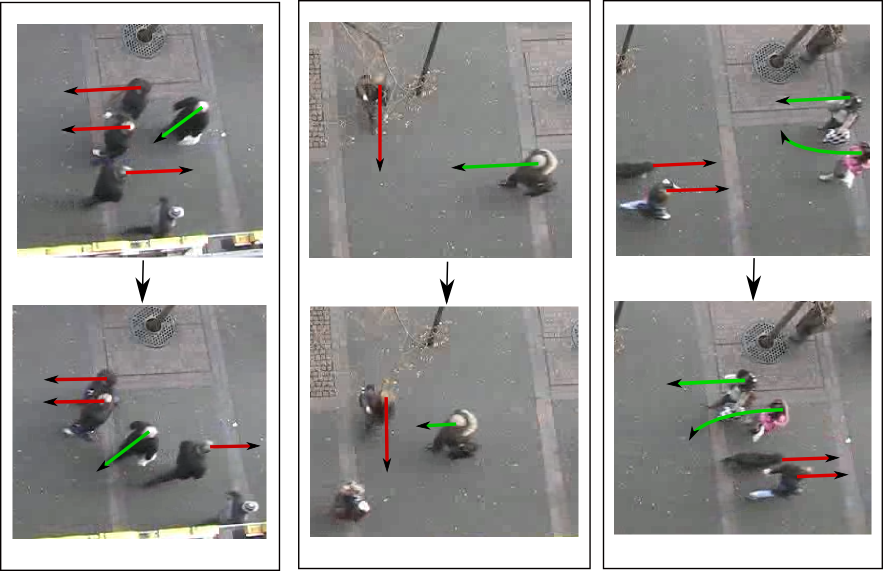
\includegraphics[width=\linewidth]{Figures/drawing-horizontal.png}
  \caption{Examples of pedestrians exhibiting cooperative behavior. In
    each image, the velocity of the pedestrian is shown as an arrow
    where the length of each arrow represents the speed. (Left) The
    pedestrian (with green arrow) anticipates the open space between
    the other three (with red arrow) and doesn't slow down. (Middle)
    The pedestrian (with green arrow) slows down to allow the other
    pedestrian (with red arrow) to pass through. (Right) The two
    pedestrians (with green arrows) make way for the oncoming agents
    (with red arrow) by going around them.}
  \label{fig:oigp-intro}
\end{figure}




The summary of our contributions in this chapter are as follows: We
develop a new algorithm for enabling robots to move naturally through
dense crowds.
Following the key insight that agents in crowd engage in \textit{joint
  collision avoidance}, we develop an approach that models the
distribution over future trajectories of all interacting agents
through a joint density model that captures the idea of
\textit{cooperative} planning, i.e., agents cooperating with each
other to achieve their goals and avoid collisions.  To capture
collision avoidance behavior, we learn a local interaction model that
encodes how agents move based on how populated their vicinity is from
real human trajectory data.  During prediction, our model infers the
goal of an agent from its past trajectory and uses the learned model
to predict its future trajectory.  Finally, we demonstrate that our
model is capable of predicting robot trajectories that are natural and
human-like by reporting the experimental results on the ETH pedestrian
video dataset~\cite{pellegrini09}.

In the remainder of this chapter, we will give an overview of relevant
existing work in section \ref{sec:oigp-related-work}. The notation and the
problem is defined in section \ref{sec:oigp-problem-definition}. Section
\ref{sec:oigp-approach} will describe our approach in detail and its
evaluation on a real world dataset is presented in section
\ref{sec:oigp-evaluation}. The results of the evaluation are discussed in
section \ref{sec:oigp-discussion} and the conclusions are presented in
section \ref{sec:oigp-conclusion}, along with directions for future work.

\section{Related Work}
\label{sec:oigp-related-work}

\subsection{Navigation in Uncertain Dynamic Environments}
\label{sec:oigp-navig-dynam-envir}
Common approaches to robot navigation in uncertain, populated environments typically compute a path to the goal without taking into account the collaborative collision avoidance behavior exhibited by humans. Most of the approaches instead rely on local reactive collision avoidance methods \cite{philippsen2003smooth, thrun99}. Although these methods effectively avoid collisions with humans, the planned trajectories are usually suboptimal, compared to the trajectory a human would take for the same start and goal, and not socially compliant due to evasive maneuvers.

Naively modeling unpredictability in the trajectories of humans, using linear models like Kalman filters, leads to increasing uncertainty that makes safe and efficient navigation difficult \cite{trautman10}. Several works have focused on controlling the uncertainty in these predictive models by developing accurate human motion models \cite{thompson09, bennewitz05}, but these approaches do not account for interactions between humans and thus cannot model joint collision avoidance. 

\subsection{Modeling human interactions}
\label{sec:oigp-inter-betw-humans}

The social forces model proposed by \cite{helbing95} models motion of pedestrians in terms of forces that drive humans to reach a goal and to avoid obstacles. Subsequently, approaches have been proposed that use learning methods to fit the social forces model to observed crowd behavior \cite{helbing09, johansson07}. The social forces model has been shown to perform well in predicting trajectories in simulated crowds, but fails when it comes to predicting movements of pedestrians in real dense crowds as it uses a hand-crafted potential term based on distances, and doesn't learn human-human interactions from real data. Using a hand-crafted potential term results in a model that can capture simple interactions, like repulsion and attractions, but may fail to account for more complex crowd behavior. \cite{adrien06} models pedestrian motion behavior using dynamic potential fields that guide people to avoid collisions and move towards the goal, but this model does not explicitly account for interactions like cooperation between agents in the crowd.

Hall \cite{hall63} introduces a theory on human proximity relationships which have been used in potential field methods to model human-human interactions \cite{svenstrup10, pradhan11}.
These models capture interactions to avoid collisions, but do not model human-robot cooperation. However,  models of cooperation are necessary for safe and efficient navigation in dense crowds \cite{trautman10}, because in cases where the crowd density is high, the robot believes there is no 
%
feasible
path in the environment unless it accounts for cooperation from the crowd. Reciprocal Velocity Obstacles (RVO), \cite{van2008reciprocal}, and Velocity Obstacles (VO), \cite{fiorini98}, account for interactions between agents by computing joint collision-free velocities assuming constant velocities and shared collision avoidance behaviors. However, these approaches cannot handle stochastic behavior in pedestrian motions and do not train the model from real observed data. 

Trautman et. al. \cite{trautman10} proposed \textit{Interacting Gaussian processes} (IGP) to explicitly model the human-robot cooperation. Similar to the work presented in this paper, IGP models the trajectories of all interacting agents jointly which results in a probabilistic model that can capture joint collision avoidance behavior. However, the IGP model assumes that the final destinations of all pedestrians are known, which is not the case in a realistic prediction task. 
%
Another drawback of IGP is the use of hand-crafted interaction potential term to model cooperative behavior which may result in robot trajectories that are not socially compliant. In this paper, we learn the interaction model from observations of real pedestrian trajectory data in the hope that we achieve more human-like and socially compliant trajectories. 

%

The works of \cite{kuderer12, Kretzschmar16} are also closely related to our work. These approaches explicitly model human-robot cooperation and jointly predict the trajectories of all agents, using feature-based representations. 
Unlike our proposed approach, they use \textit{maximum entropy inverse reinforcement learning} (IRL) to learn an interaction model from human trajectory database using carefully designed features 
%
such as clearance, velocity, or group membership.
However, their approach has been tested in scripted environments with no more than four humans. In our work, we deal with crowded scenarios with an average of six humans in a single scene. Very recently, \cite{pfeiffer16} have extended the maximum entropy approach to unseen and unstructured environments by using a receding horizon motion planning approach.
%

\subsection{Trajectory prediction}
\label{sec:oigp-traj-pred}

A large body of works exist in the domain of computer vision and video surveillance that deal with predicting motion of people in videos, that are relevant to our work. \cite{kim11, joseph2011bayesian} learn motion patterns using Gaussian processes and cluster human trajectories into these motion patterns. But these approaches ignore human-human interactions. IRL has also been used in the domain of activity forecasting to predict human paths in static scenes, \cite{kitani2012activity} and more recently, \cite{alahi16} used Long Short-Term Memory networks (LSTM) to jointly reason across multiple agents to predict their trajectories in a scene. However, most of these approaches have been used in the context of prediction and have not been extended to navigation.

\section{Problem Definition}
\label{sec:oigp-problem-definition}

\subsection{Notation}
\label{sec:oigp-notation}

We follow the notation of \cite{trautman10}.
Let the index $i \in \{1,2,\cdots,N\}$ specify the agent, where $N$ is the number of individuals in the crowd and $i=R$ indicates the robot. 
The trajectory of agent $i \in \{R,1,2,\cdots,N\}$ is given by $\fbold\supi$ $= (f_1^{(i)}, f_2^{(i)}, \cdots, f_T^{(i)})$, where $T$ is the length of the trajectory and $f_t^{(i)} = (x_t^{(i)}, y_t^{(i)}) \in \mathbb{R}^2$ is the location of agent $i$ at time-step $t$. The observed locations of pedestrian $i$ until time-step $t$ is denoted as $\zbold\supi\subt = (z_1^{(i)}, z_2^{(i)}, \cdots, z_t^{(i)})$.  We denote the set of all pedestrian trajectories by $\fbold=\{\fbold\supi\}_{i=1:N}$, the robot trajectory by $\fbold\supR$, and the set of all pedestrian observations until time-step $t$ by $\zbold\subt = \{\zbold\supi\subt\}_{i=1:N}$. We assume a fixed number of goals $g$ in the environment are known and denote the set of goals by $\Gbold$. %

\subsection{Planning using the joint density}
\label{sec:oigp-planning}
%
%
%
%
Following the assumption that people engage in a joint collision
avoidance when moving through a dense crowd
 as in \cite{helbing95,trautman10},
the robot does not only have to respond to the observed trajectories
of the pedestrians, but also has to account for the adaptive behavior
of the humans.

To capture this cooperative behavior, it has been suggested by
~\cite{trautman10} to use the joint density of both the robot and the
crowd, denoted by $P(\fbold\supR, \fbold|\zbold\subt)$.
%
%
%
%
%
Planning the path for the robot using this density corresponds to
finding the maximum-a-priori (MAP) assignment for the following
posterior:
\begin{equation}
  \label{eq:oigp-8}
  (\fbold\supR, \fbold)_* = \argmax_{\fbold\supR, \fbold} P(\fbold\supR, \fbold|\zbold\subt).
\end{equation}

%
%
%
%
%
%
%

\subsection{Problem}
\label{sec:oigp-problem}
In this work, we assume that at each time-step $t$, we receive the observation $\zbold_t$ of the locations of all agents in the crowd. Given the current and past observations $\zbold\subt$, we tackle the problem of estimating the joint posterior distribution of the future trajectories of all agents. Formally, we seek to model the density given by,
$$ P(\fbold\supR, \fbold | \zbold\subt).$$
%
Planning the robot's trajectory then corresponds to taking the MAP assignment for $\fbold\supR$ and executing it until the next observation is received. At time-step $t+1$, we receive a new observation $\zbold_{t+1}$ and update the above joint posterior density to $P(\fbold\supR, \fbold|\zbold_{1:t+1})$. This process is repeated until the robot reaches its destination. 
%
In contrast to \cite{trautman10}, who tackle a similar problem, we aim to predict more natural and human-like robot trajectories by learning the model from pedestrian trajectory data. 

%

%

%
%
%
%

\section{Approach}
\label{sec:oigp-approach}

\begin{figure}[t!]
  \centering
  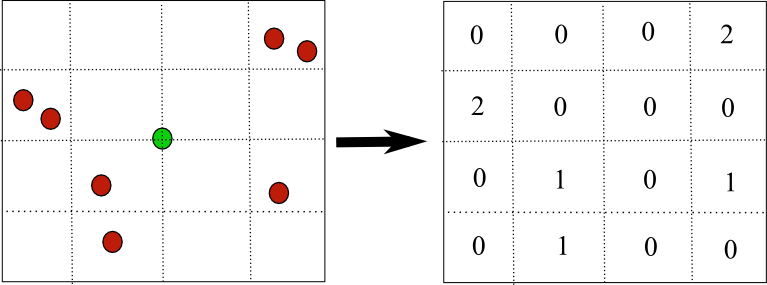
\includegraphics[width=\linewidth]{Figures/ogrid-sharp.png}
  \caption{Occupancy grid construction. (Left) A configuration of
    other agents (red) around the current agent (green). (right) 4x4
    occupancy grid is constructed using the number of agents in each
    grid cell}
  \label{fig:oigp-ogrid}
\end{figure}

We exploit the observation that humans navigating in dense crowds
adapt their trajectories based on the presence of agents in their
vicinity \cite{alahi16}.
%
%
%
%
We first explain the construction of \textit{occupancy grids}, which
account for the presence of other agents within an agent's local
neighborhood (Section \ref{sec:oigp-occupancy}).  We formulate the problem
of learning the social interaction model as a Gaussian process
regression problem, where we predict the agent's velocities at each
time-step as a function of their occupancy grids and intended
goal. Given the preprocessed training trajectories (Section
\ref{sec:oigp-preprocessing}), we train the GP model by maximizing its
marginal likelihood to learn the hyperparameters of the kernel
(Section \ref{sec:oigp-train}). At prediction time, we use the learned
model to infer the goal of each agent and jointly predict future
trajectories of all interacting agents in the crowd (Section
\ref{sec:oigp-prediction}).

\subsection{Constructing occupancy grids}
\label{sec:oigp-occupancy}
To capture the local interactions of an agent with its neighbors, we
construct an occupancy grid for each agent $i$ at each time-step $t$
that is similar to the social pooling grid used in \cite{alahi16}. The
occupancy grid is constructed by discretizing the neighborhood of the
agent's current location into a spatial grid of size $M \times M$. We
then count the number of surrounding agents within each grid
cell. Formally, we define occupancy grid as a vector of length $M^2$
given by,
\begin{equation}
  \label{eq:oigp-2}
  \Obold_t\supi (a + M(b-1)) = \sum_{j \in \mathcal{N}\supi}\mathbb{I}_{a,b}[x_t\supj - x_t\supi, y_t\supj - y_t\supi].
\end{equation}
$\mathcal{N}\supi$ denotes the set of all agents $j \neq i$, who are
within the neighborhood of agent $i$. The indicator function
$\mathbb{I}_{a,b}[x,y]$ defines if $(x,y)$ is located in the $(a,b)$
cell of the occupancy grid.
%
%
In the remainder of the paper, $\Obold\supi$ and $\Obold$ will denote
the set of all occupancy grids at every time-step of an agent $i$ and
that of all agents, respectively.
%
%
%

%
\subsection{Preparing training data for learning}
\label{sec:oigp-preprocessing}

%
%
%
%
%
%
%
%
%
%

%
%
%
%
%
%
Before training our model, we preprocess the training data $\fbold$,
which correspond to the trajectories of all agents. First, we
construct occupancy grids $\Obold\supi$ and $\Obold$ along $\fbold$, as described in
Section \ref{sec:oigp-occupancy}. Second, we process all the trajectories
to obtain the velocities of agents at each time-step $(\xvel,
\yvel)$. Third, since we have access to the entire trajectory at
training, we can compute the goals of all the pedestrians.  Note that
this information about the true goals is used only during training and
is not assumed in the prediction phase.  After this preprocessing, we
have $(\Obold, \xbvel, \ybvel)$ for all agents at every time-step and
their corresponding goals $\{g\supi\}$.%

\subsection{Training the local interaction model}
\label{sec:oigp-train}

To learn across different pedestrians traversing in different regions
of the environment, we model the velocity of an agent at a specific
time-step as a function of their intended goal and their occupancy
grid at that time-step. Formally, we seek to estimate the distribution
$P(\xbvel| \Obold, g)$ and $P(\ybvel| \Obold, g)$, for each goal $g$
in $\Gbold$, from the training data obtained in Section
\ref{sec:oigp-preprocessing}.

We start by modeling the interactions as a Gaussian Process (GP)
regression problem, where the noisy data to be interpolated is
$(\Obold, \xbvel)$ and $(\Obold, \ybvel)$. Note that we use a separate
GP for each goal $g$ to learn the mapping from occupancy grids to
velocities. We use a \textit{squared exponential automatic relevance
  determination} (SE-ARD) kernel (with additive noise) for these GPs
\cite{rasmussen06}.  The SE-ARD kernel learns a different lengthscale
for each input dimension, which in our problem are the dimensions of
the occupancy grid vector, i.e., the grid cells. Since, the kernel can
learn the relevance of each input dimension by learning the
lengthscale parameter \cite{rasmussen06} (dimensions with large
lengthscales are less relevant than those with small lengthscales), the
kernel will capture the relevance of each grid cell for a specific
goal and effectively ignore irrelevant cells.
%
%
%
%
%
%
%
%
%
%
%
%


The SE-ARD kernel with additive noise is given by,
\begin{align}
  \label{eqn:oigp-kernel}
  \begin{split}
    K_{S}(\Obold, \Obold') &= \sigma_f^2 \exp\left(-\frac{1}{2}\sum_{d=1}^{M^2} \frac{(\Obold(d) - \Obold'(d))^2}{\ell_d^2}\right) \\
    &+ \sigma_n^2 \delta(\Obold, \Obold')
  \end{split}
\end{align}
where $\delta(\Obold,\Obold') = 1$ if $\Obold$ is equal to $\Obold'$
and zero otherwise, and $\Obold(d)$ is the value of the $d^{th}$
dimension in the vector $\Obold$. The hyperparameters of this kernel
are $\sigma_f$ (signal variance), $\{\ell_d\}_{d=1}^{M^{2}}$
(lengthscales) and $\sigma_n$ (noise variance).


This construction results in a total of $2G$ GPs because there is a
pair of GPs (in x- and y-direction) for each of the $G$ goals; thus,
we have $2G$ sets of hyperparameters to be learned. We denote the set
of hyperparameters corresponding to the GP associated with goal $g$ by
$\Theta_x^g$ and $\Theta_y^g$. To learn the hyperparameters
$\Theta_x^g$, we isolate the tuples
$B_g = \{(\Obold\supi, \xbvel\supi)\}_i$ from training data,
corresponding to the set of pedestrians $i$ whose goal is $g$, and
maximize the log marginal likelihood of the GP \cite{rasmussen06}
given by,
%
%

\begin{align}
  \label{eqn:oigp-logmarginal}
  \begin{split}
    \log P\left(\xbvel|\Obold\right) &= -\frac{1}{2}\xbvel^TK_S(\Obold, \Obold)^{-1}\xbvel \\
    &- \frac{1}{2}\log|K_S(\Obold, \Obold)| - \frac{n_g}{2}\log 2\pi
  \end{split}
\end{align}
where $\xbvel$ and $\Obold$ are vectors constructed by concatenating
elements of $B_g$, and $n_g$ is the number of elements in $\xbvel$.

We can learn $\Theta_y^g$ and all the other sets of hyperparameters
for all goals $g \in \Gbold$ in a similar fashion.
%
%
%
%
%

\subsection{Prediction}
\label{sec:oigp-prediction}

During prediction we are given an unseen crowd with $N_p$ pedestrians,
a robot, and their observations $\zbold_{1:t}$ until time $t$. Our
task is to predict their trajectories $\fbold$ and $\fbold\supR$ for
$H$ time-steps into the future, using the learned model. We cannot
directly use the GP predictive distribution because we do not know the
goals of the pedestrians during prediction. Note that we know the goal
of the robot $g\supR$ since it is user-defined.

\subsubsection{Infer goal of a pedestrian}
\label{sec:oigp-infer}

Given observations $\zbold\supi\subt$ of pedestrian $i$ until time $t$
and the set of goals $\Gbold$, we seek to infer the goal
$g\supi \in \Gbold$ of the pedestrian. We assume a uniform prior
$P(g\supi)$ over all goals, in the absence of any observations for
agent $i$ (A more informative prior over the goals can be found by
analyzing the environment). Hence, we have:
\begin{equation}
  \label{eq:oigp-1}
  P(g\supi|\zbold\supi\subt) = \frac{P(\zbold\supi\subt|g\supi) P(g\supi)}{P(\zbold\supi\subt)} \propto P(\zbold\supi\subt|g\supi).
\end{equation}

That is, we evaluate the likelihood that the observation sequence
$\zbold\supi\subt$ is true conditioned on the fact that $g\supi$ is
the goal of agent $i$. Similar approaches have been explored in
\cite{kitani2012activity} and \cite{ziebart09}, for inferring destination of an
agent given its previous path.
 
%
%
%
%
%
%
%
%
%
To compute the likelihood, we first compute, from the observations
$\zbold\subt$, the velocities $\{(\xbvel, \ybvel)\}_{1:t-1}$ and the
occupancy grids $\Obold_{1:t-1}$ of all pedestrians at each time-step
until $t-1$.  For each possible goal $g \in \Gbold$, we take the
corresponding set of trained hyperparameters $\Theta_x^g$ and
$\Theta_y^g$, and evaluate the log marginal likelihood of the GP for
each agent $i$ (using equation \ref{eqn:oigp-logmarginal}).
%
%
%
%
Hence, for each agent $i$ and each goal $g\supi \in \Gbold$, we obtain
the likelihood that its observed data $\zbold\supi\subt$ is generated
from the GP conditioned on the goal $g\supi$. Normalizing the
likelihoods across all goals, we get the likelihood
$P(\zbold\subt\supi|g\supi)$ for every goal $g\supi \in \Gbold$.


\subsubsection{Predicting future trajectories}
\label{sec:oigp-pred-future-traj}

Now that we have a distribution over the goals $g\supi$ for all agents
$i$ in the crowd, we can use the trained model to predict future
locations. The joint posterior density can be decomposed as
\begin{equation}
  \label{eq:oigp-11}
  P(\fbold\supR, \fbold | \zbold\subt) = \sum_{\gbold} P(\fbold\supR, \fbold | \gbold, \zbold\subt) P(\gbold | \zbold\subt)
\end{equation}
where $\gbold = \{g\supi\}_{i=R,1:N}$ are the goals of all agents
including the robot.
%
%
We can assume that the goals of the pedestrians are independent of
each other (and that we know the goal of the robot with certainty)
given their respective observations. Then, we can write the
distribution of a goal given a history of observations as:
\begin{equation}
  \label{eq:oigp-12}
  P(\gbold|\zbold\subt) = \prod_{i=1}^{N} P(g\supi|\zbold\subt\supi)
\end{equation}
where $P(g\supi|\zbold\subt\supi)$ is given by equation \ref{eq:oigp-1}.
We approximate the joint distribution
$P(\fbold\supR, \fbold|\gbold, \zbold\subt)$ by using the velocities
and occupancy grids obtained from observations $\zbold\subt$ (as done
in Section \ref{sec:oigp-infer}),
\begin{equation}
  \label{eq:oigp-13}
  %
  %
  %
  P(\fbold\supR, \fbold|\gbold, \zbold\subt) \approx P(\fbold\supR, \fbold|\{\xbvel, \ybvel\}_{1:t-1}, \Obold\subt, \gbold)
\end{equation}
%
%
The predictions for different agents are coupled through the occupancy
grid which contains the configuration of other agents around each
agent locally.
%
%
%
%
This enables our model to capture local interactions, like joint
collision avoidance and cooperation.

Since the task is to predict the future locations of all agents for
the next $H$ time-steps, $\fbold\supi$ suffices to represent the next
$H$ locations of agent $i$ after time $t$, in addition to previous
locations.

\subsubsection{Multi-step prediction}
\label{sec:oigp-sampling}
Future locations can be predicted using the learned model from Section
\ref{sec:oigp-train}. For each agent $i$, we fit a separate pair of GPs
(with the learned hyperparameters $\Theta_x^g$, $\Theta_y^g$ for goal
$g$) to the observed tuples $(\Obold\supi\subt, \{\xbvel\}\subti\supi)$
and $(\Obold\supi\subt, \{\ybvel\}\subti\supi)$. Using their
corresponding GPs, each agent can predict their velocities and compute
the location for the next time-step by adding it to the current
location.

This can be done exactly for time $t+1$, i.e., we can predict
$(\xbvel)_{t+1}\supi$ and $(\ybvel)_{t+1}\supi$ for each agent $i$,
since we know the value of the occupancy grid at time $t$,
$\Obold\supi_t$. But for future time-steps, we need to estimate the
occupancy grid at the previous time step using previous
predictions. Instead of computing the distribution over future
locations in an exact form (which can be extremely difficult), we use
Monte Carlo sampling to approximate the distribution as shown in
Algorithm \ref{alg:oigp-sampling}.

At time $t+1$, we compute the GP predictive distribution
\cite{rasmussen06} for each $(\xbvel)_{t+1}\supi$ and
$(\ybvel)_{t+1}\supi$ (line \ref{alg:line:start}).
We then proceed to sample $S$ points from each of these distributions
(line \ref{alg:line:sample}), and estimate $S$ samples for the
location $\fbold_{t+1}\supi$ for all agents $i$ (line
\ref{alg:line:estimate}).  These sets of samples approximate the
distribution
$P(\fbold\supR_{t+1}, \fbold_{t+1}|\{\xbvel, \ybvel\}_{1:t-1},
\Obold\subt, \gbold)$.

Since, for each sample, we have locations of all agents at time $t+1$,
we can compute occupancy grids $\Obold\supi_{t+1}$ for each agent
(line \ref{alg:line:estimateocc}). Thus, we get $S$ samples for
$\Obold_{t+1}$.  Now, to estimate location at time $t+2$, we compute
the mean of the $S$ samples to get the set of occupancy grids,
$\Obold_{t+1}$ (line \ref{alg:line:mean}).  Using the mean,
%
we predict the velocities at time $t+2$ (line \ref{alg:line:repeat}),
and repeat the above process until $H$ time-steps into the future. At
every time-step $t'$ ($t' \geq t+1, t' \leq t+H$), we get a set of $S$
samples corresponding to the locations $\fbold_{t'}$ that approximate
the distribution
\begin{align*}
  \{\fbold\supR_{t'}, \fbold_{t'}\}_{j=1:S} \approx P(\fbold\supR_{t'}, \fbold_{t'}|\{\xbvel, \ybvel\}_{1:t-1}, \Obold\subt, \gbold)
\end{align*}
As we let the value of $S$ grow, we get a better approximation.


\begin{algorithm}[h]
  \begin{algorithmic}[1]
    \For{each agent $i$} \State Compute distributions of
    $(\xbvel)_{t+1}\supi$, $(\ybvel)_{t+1}\supi$ given
    $\Obold\supi_t$\label{alg:line:start}
    \EndFor
    \For{$t'=t+2 \to t+H$} \For{each agent $i$} \State Sample $S$
    points from distributions of $(\xbvel)_{t'-1}\supi$,
    $(\ybvel)_{t'-1}\supi$\label{alg:line:sample} \State Compute $S$
    estimates for $\fbold\supi_{t'}$ from sampled
    velocities\label{alg:line:estimate}
    \EndFor
    \State Compute $S$ samples for $\Obold_{t'}$ from estimates of
    $\fbold_{t'}$\label{alg:line:estimateocc} \State Set $\Obold_{t'}$
    to be the mean of the $S$ samples from above \label{alg:line:mean}
    \For{each agent $i$} \State Compute distributions of
    $(\xbvel)_{t'}\supi$, $(\ybvel)_{t'}\supi$ given
    $\Obold\supi_{t'}$\label{alg:line:repeat}
    \EndFor
    \EndFor \\
    \Return
    $\{\{\fbold\supR_{t'},
    \fbold_{t'}\}_{j=1:S}\}_{t'=t+1:t+H}$\label{alg:line:return}
  \end{algorithmic}
  \caption{Multi-step prediction through Sampling}
  \label{alg:oigp-sampling}
\end{algorithm}



\section{Evaluation}
\label{sec:oigp-evaluation}

\subsection{Setup}
\label{sec:oigp-setup}

We evaluate our model on a publicly available human-trajectory dataset
released by ETH, \cite{pellegrini09}.
%
%
%
%
The dataset contains a video recorded from above a busy doorway of a
university building with the pedestrian trajectories tracked and
annotated.  This video contains scenes with real world crowded
settings, hundreds of trajectories and high crowd density.
%
%
%
%
%
An example snapshot from the video (with goals marked) is shown in
figure \ref{fig:oigp-snapshot}. Each time-step in the video is six frames
long and amounts to 0.4 seconds. The average trajectory length of a
pedestrian is 25 time-steps. The total number of pedestrians in the
video is 360 and there are four goals in the environment. The
resolution of the video is $640 \times 480$. Each pixel in the video
frame corresponds to 0.042 metres (slightly varies across the frame,
as the camera is angled and not exactly top-down).

%
%
%
%
%
%
%
%
%
%
%

We evaluate our model by choosing a pedestrian in the crowd randomly
as our robot and use his start and goal state to plan a path through
the crowd. The resulting path is compared to the true path that the
pedestrian has taken in the video. Comparing the true path and the
predicted path gives us a evaluation of how closely our prediction
resembles human-like behavior. A similar evaluation was done in
\cite{trautman10}.

%
%
%
%
%
%
%
%
%
%
%
%
%
%
%
%
%
%

\begin{figure}[t!]
  \centering
  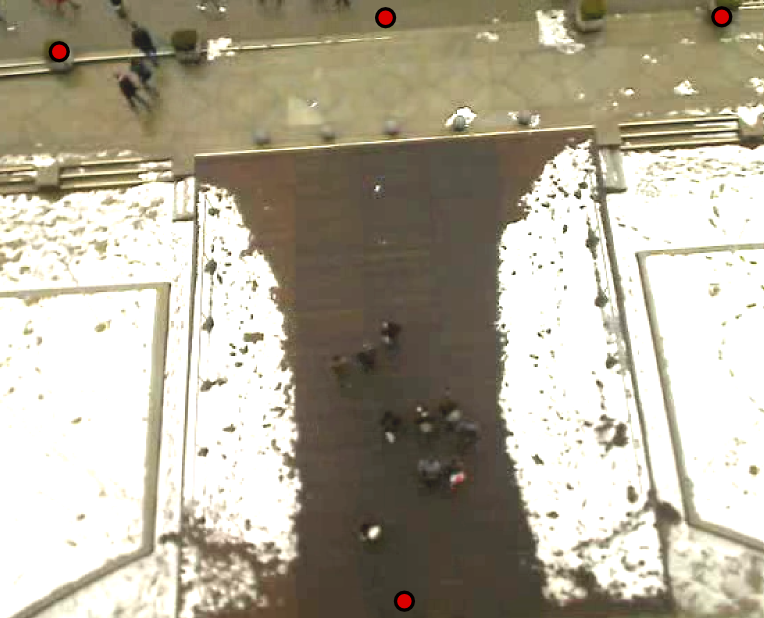
\includegraphics[width=0.7\linewidth]{Figures/snap-label.png}
  \caption{Example snapshot of the dataset with goals indicated by red
    dots}
  \label{fig:oigp-snapshot}
\end{figure}

We compare our approach against IGP \cite{trautman10}, as it deals
with the same problem of jointly modeling trajectories of robot and
pedestrians, and has shown good results in real robot navigation
scenario among dense crowds \cite{trautman13, trautman15}.
%
%
%
%
%
%
We will use both our approach and IGP to predict the path until $H$
time-steps into the future and compare it with the true trajectory.

Note that the original IGP needs to know the true final destination of
each pedestrian at prediction time, which would give it an unfair
advantage over our algorithm. Hence, we use a variant of IGP which
doesn't need the true final destinations and use that in our
comparison. At prediction time, we compute the average heading of the
pedestrian for the last 5 time-steps and estimate the goal location in
the computed heading direction. The estimated goal is used in the
original IGP algorithm in place of the true final destination of the
pedestrian.
%
%
%

To compare the path predicted by the two algorithms and the true path
of the pedestrian, we consider two metrics:
\begin{enumerate}
\item \textit{Average displacement error}: Introduced in
  \cite{pellegrini09}, this metric computes the mean squared error
  over all estimated points at each time-step in the predicted
  trajectory and the true trajectory.
\item \textit{Final displacement error}: Introduced in \cite{alahi16},
  this metric computes the mean distance between the final predicted
  location after $H$ time-steps and the true location after $H$
  time-steps, where $H$ is our prediction horizon.
\end{enumerate}

\subsection{Model Parameters}
\label{sec:oigp-model-parameters}

We construct occupancy grids around each agent of size $4 \times 4$ (i.e. $M=4$) covering a space of $80 \times 80$ pixels in the video. In each video, we train the model on the trajectories of the first 50 pedestrians. At prediction time, we chose a scenario with 11 pedestrians (from the remaining part of the video, not used in training), one of whom is used as a robot in our model. We predict the future locations for a range of prediction horizons $H = 1,2,5,10,20$ time-steps. If the path of the pedestrian (or robot) ends in less than $H$ time-steps, we will predict only until the end of his path. For multi-step prediction, we use $S = 100$ samples to approximate the distribution over future locations. We implement the Gaussian process regression model using the GPML toolbox, \cite{rasmussen06}.


\subsection{Results}
\label{sec:oigp-results}

\begin{figure}[t!]
  \centering
  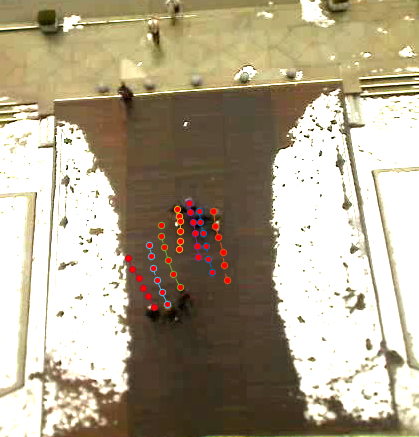
\includegraphics[width=0.7\linewidth]{Figures/igp2-crop.png}
  \caption{Example prediction by our model. For each pedestrian, we predict his future locations (which are plotted) for the next 5 time-steps. The bottom set of pedestrians are progressing towards a goal at the top centre of the image, but they go around the other set of pedestrians making way for them cooperatively}
  \label{fig:oigp-bestcase}
  %
\end{figure}

To test the prediction accuracy of both approaches, we have chosen scenarios with 11 pedestrians in the crowd where crowd density is high and some pedestrians head into and through the crowd. To get an unbiased estimate, we chose 5 such scenarios in the video. In each scenario, we assume each pedestrian to be the robot, one at a time, and compute their average displacement error and final displacement error, averaged over all time-steps. This results in 11 sets of error values and we compute the average over all sets to give the mean errors over all pedestrians. We repeat the experiment for different $H$ values to get both short-range and long-range prediction accuracies of both approaches. The results are averaged over all 5 scenarios and are presented in Table \ref{table:oigp-results}. Note that the errors are listed in pixels.

\begin{table}[t!]
  \caption{Prediction errors (in pixels) on the dataset for IGP and our approach}
  \centering
  \begin{tabular}{|c|c|c|c|}
    \hline
    Metric & Prediction horizon ($H$) & IGP & Our Approach \\
    \hline
    \multirow{5}{*}{Avg. Disp. Error} & 1 & 3.42 & 4.42 \\
    & 2 & 5.66 & 6.14 \\
    & 5 & 15.75 & 12.09 \\
    & 10 & 21.59 & 21.52 \\
    & 20 & 41.51 & 34.63 \\
    \hline
    \multirow{5}{*}{Final Disp. Error} & 1 & 3.42 & 4.42 \\
    & 2 & 7.12 & 7.78 \\
    & 5 & 23.18 & 19.77 \\
    & 10 & 38.75 & 36.25 \\
    & 20 & 67.41 & 54.2 \\
    \hline
  \end{tabular}
  \label{table:oigp-results}
\end{table}

In Figure \ref{fig:oigp-bestcase}, we show an example scene where our approach predicts cooperative behavior. The set of pedestrians going up give way to the set of pedestrians going down. To visualize what our local interaction model (from section \ref{sec:oigp-train}) learned, we give it some example occupancy grids and goals, and observe the predicted velocities. Figure \ref{fig:oigp-learnedmodel} shows that the model learns collision avoidance as it predicts velocities away from grid cells which are occupied and towards unoccupied grid cells. When an agent's vicinity is heavily populated in the direction of its goal, the magnitude of predicted velocity is very low, i.e., the agent moves slowly. If instead, its vicinity is populated in the opposite direction of its goal, the velocity of the agent doesn't get affected by the surrounding agents (as they are not obstructing its path).

To verify this observation, we have examined the values of the learned hyperparameters of the SE-ARD kernel. The lengthscales for grid cells that are not in the direction of the pedestrian's intended goal, are given high values, thus reducing their relevance in the velocity prediction. For example, in Figure \ref{fig:oigp-learnedmodel} the lengthscales for the bottom grid cells in the left bottom occupancy grid, are set to values higher than 7 whereas the lengthscales for the top grid cells in the same grid are set to values lower than 1. This shows that our model learns how neighbors affect a pedestrian's path based on their relative spatial orientation. 

\begin{figure}[t!]
  \centering
  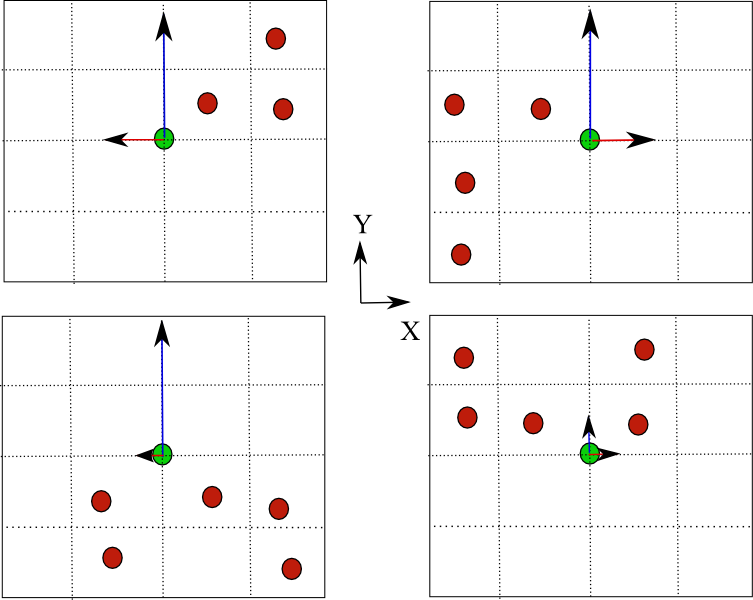
\includegraphics[width=\linewidth]{Figures/sample-ogrid.png}
  \caption{Velocities predicted by our trained model for example occupancy grids. In each case, the goal of the pedestrian is right above in the Y-direction. Predicted mean y-velocity is shown in blue and predicted mean x-velocity is shown in red.}
  \label{fig:oigp-learnedmodel}
\end{figure}

\section{Discussion}
\label{sec:oigp-discussion}

From the results presented in Table \ref{table:oigp-results}, we can
observe that our approach performs better than IGP at predicting human
trajectories for longer prediction horizons and worse for shorter
horizons. This is mainly because IGP models trajectories directly by
predicting future locations based on previously observed locations. This
results in very accurate predictions in situations where there are no
surrounding agents (and hence, no interactions) and for shorter
prediction horizons, as it extrapolates the trajectory to future
time-steps smoothly. Our model, on the other hand, models velocities
at each time-step and needs to estimate the future location based on
velocity predictions for the previous time-step. Thus, for shorter
prediction horizons, our model has a higher variance associated with
predicted locations. But for longer horizons, our model has higher
accuracy in prediction as it reasons about the intended goal of the
agent and captures local interactions at each time-step. IGP fails at
longer horizons as the smooth extrapolation, coupled with the
handcrafted interaction potential term, is unable to account for all
the interactions and cooperative behavior among dense crowds. More
importantly, our approach has a higher performance than IGP because it
learns the local interaction model from real human trajectory data
whereas the interaction model in IGP is hand-crafted.

Accurate predictions for longer horizons is important in social navigation
as it results in a more globally optimal behavior. In cases where the
prediction is accurate in a short horizon but poor for longer horizons,
the resulting paths are locally optimal and can potentially lead to a
non-socially compliant and reactive behavior.

Upon careful examination of predictions of our approach in crowded
scenarios, we observed that it learns the behavior of slowing down
(see bottom right of Figure \ref{fig:oigp-learnedmodel}) when its vicinity
is heavily populated, which is a common behavior among humans. Also,
as observed from the values of the learned lengthscales for the SE-ARD
kernel, our model learns how humans decide their velocity based on the
relative spatial configuration of other agents in their
neighborhood. As shown in Figure \ref{fig:oigp-learnedmodel}, our trained
local interaction model captures collision avoidance based on an
agent's occupancy grid by learning from human trajectory data without
any hand-crafted potential term.

Although we present results for predicting trajectories of every
agent in the crowd, this approach can be extended to robot navigation by
treating the robot as an agent in the crowd. Planning the path of the
robot in this model reduces to inference in the joint density as shown
in Section \ref{sec:oigp-planning}. The resulting path taken by the robot
is the most likely path predicted according to the learned
model. Recent work by \cite{pfeiffer16} has shown that as long as
pedestrians interact with the robot naturally (as one of them), such
an interaction-aware modeling approach is significantly better than a
reactive approach.


\section{Summary}
\label{sec:oigp-conclusion}

In this chapter, we presented a new approach to modeling cooperative
behavior among humans in dense crowds. While most existing approaches
use hand-crafted models to capture interactions among humans in the
crowd, we take a data-driven approach and learn an interaction model
from real human trajectory data. We propose a nonparametric
statistical model that uses Gaussian processes to model velocities of
agents in the crowd as a function of how populated their vicinity
is. We show how our model can be used to predict future trajectories
of pedestrians and compute the path of a robot through a dense
crowd. The future trajectories are computed using a Monte Carlo
sampling approach to multi-step prediction. Lastly, the efficacy of
our approach is demonstrated by predicting trajectories of agents in a
real world pedestrian dataset. Our results show that the model
captures important aspects of human crowd behavior such as cooperative
navigation and collision avoidance.

 Another important drawback of our
approach is the assumption of known goals in the environment. This
restricts the generalizability of the approach to previously seen
environments and a separate model needs to be trained for a new
environment.


%As a part of future work, we plan to validate and verify our approach
%on a real robot placed in a dense human crowd. The task would be,
%given a start and goal location, the robot should be able to navigate
%safely and efficiently through the crowd. In addition to validating
%our approach, we intend to tackle the drawbacks of the approach as
%stated before. We are also looking to extend the model by coming up
%with latent representations of trajectories that encode time-varying
%information such as pedestrian's intention, planned future path and
%velocities, that can be used instead of an occupancy grid in our
%approach.


%%% Local Variables:
%%% mode: latex
%%% TeX-master: "thesis"
%%% End:


\clearpage

\chapter{Attention in Human Crowds}
\label{chap:attn}

%%% Local Variables:
%%% mode: latex
%%% TeX-master: "thesis"
%%% End:


\clearpage

\chapter{Conclusion}
\label{chap:conclusion}
\note{Conclude the thesis. Sections should be: \textbf{Summary} and \textbf{Future Work}.}
%%% Local Variables:
%%% mode: latex
%%% TeX-master: "thesis"
%%% End:


%Include references using bst and bib files.
\bibliographystyle{finitplain} 
{\small \bibliography{local}}


\end{document}

%%% Local Variables:
%%% mode: latex
%%% TeX-master: t
%%% End:
